% Options for packages loaded elsewhere
\PassOptionsToPackage{unicode}{hyperref}
\PassOptionsToPackage{hyphens}{url}
\PassOptionsToPackage{dvipsnames,svgnames,x11names}{xcolor}
%
\documentclass[
  letterpaper,
  DIV=11,
  numbers=noendperiod]{scrartcl}

\usepackage{amsmath,amssymb}
\usepackage{iftex}
\ifPDFTeX
  \usepackage[T1]{fontenc}
  \usepackage[utf8]{inputenc}
  \usepackage{textcomp} % provide euro and other symbols
\else % if luatex or xetex
  \usepackage{unicode-math}
  \defaultfontfeatures{Scale=MatchLowercase}
  \defaultfontfeatures[\rmfamily]{Ligatures=TeX,Scale=1}
\fi
\usepackage{lmodern}
\ifPDFTeX\else  
    % xetex/luatex font selection
\fi
% Use upquote if available, for straight quotes in verbatim environments
\IfFileExists{upquote.sty}{\usepackage{upquote}}{}
\IfFileExists{microtype.sty}{% use microtype if available
  \usepackage[]{microtype}
  \UseMicrotypeSet[protrusion]{basicmath} % disable protrusion for tt fonts
}{}
\makeatletter
\@ifundefined{KOMAClassName}{% if non-KOMA class
  \IfFileExists{parskip.sty}{%
    \usepackage{parskip}
  }{% else
    \setlength{\parindent}{0pt}
    \setlength{\parskip}{6pt plus 2pt minus 1pt}}
}{% if KOMA class
  \KOMAoptions{parskip=half}}
\makeatother
\usepackage{xcolor}
\setlength{\emergencystretch}{3em} % prevent overfull lines
\setcounter{secnumdepth}{-\maxdimen} % remove section numbering
% Make \paragraph and \subparagraph free-standing
\makeatletter
\ifx\paragraph\undefined\else
  \let\oldparagraph\paragraph
  \renewcommand{\paragraph}{
    \@ifstar
      \xxxParagraphStar
      \xxxParagraphNoStar
  }
  \newcommand{\xxxParagraphStar}[1]{\oldparagraph*{#1}\mbox{}}
  \newcommand{\xxxParagraphNoStar}[1]{\oldparagraph{#1}\mbox{}}
\fi
\ifx\subparagraph\undefined\else
  \let\oldsubparagraph\subparagraph
  \renewcommand{\subparagraph}{
    \@ifstar
      \xxxSubParagraphStar
      \xxxSubParagraphNoStar
  }
  \newcommand{\xxxSubParagraphStar}[1]{\oldsubparagraph*{#1}\mbox{}}
  \newcommand{\xxxSubParagraphNoStar}[1]{\oldsubparagraph{#1}\mbox{}}
\fi
\makeatother

\usepackage{color}
\usepackage{fancyvrb}
\newcommand{\VerbBar}{|}
\newcommand{\VERB}{\Verb[commandchars=\\\{\}]}
\DefineVerbatimEnvironment{Highlighting}{Verbatim}{commandchars=\\\{\}}
% Add ',fontsize=\small' for more characters per line
\usepackage{framed}
\definecolor{shadecolor}{RGB}{241,243,245}
\newenvironment{Shaded}{\begin{snugshade}}{\end{snugshade}}
\newcommand{\AlertTok}[1]{\textcolor[rgb]{0.68,0.00,0.00}{#1}}
\newcommand{\AnnotationTok}[1]{\textcolor[rgb]{0.37,0.37,0.37}{#1}}
\newcommand{\AttributeTok}[1]{\textcolor[rgb]{0.40,0.45,0.13}{#1}}
\newcommand{\BaseNTok}[1]{\textcolor[rgb]{0.68,0.00,0.00}{#1}}
\newcommand{\BuiltInTok}[1]{\textcolor[rgb]{0.00,0.23,0.31}{#1}}
\newcommand{\CharTok}[1]{\textcolor[rgb]{0.13,0.47,0.30}{#1}}
\newcommand{\CommentTok}[1]{\textcolor[rgb]{0.37,0.37,0.37}{#1}}
\newcommand{\CommentVarTok}[1]{\textcolor[rgb]{0.37,0.37,0.37}{\textit{#1}}}
\newcommand{\ConstantTok}[1]{\textcolor[rgb]{0.56,0.35,0.01}{#1}}
\newcommand{\ControlFlowTok}[1]{\textcolor[rgb]{0.00,0.23,0.31}{\textbf{#1}}}
\newcommand{\DataTypeTok}[1]{\textcolor[rgb]{0.68,0.00,0.00}{#1}}
\newcommand{\DecValTok}[1]{\textcolor[rgb]{0.68,0.00,0.00}{#1}}
\newcommand{\DocumentationTok}[1]{\textcolor[rgb]{0.37,0.37,0.37}{\textit{#1}}}
\newcommand{\ErrorTok}[1]{\textcolor[rgb]{0.68,0.00,0.00}{#1}}
\newcommand{\ExtensionTok}[1]{\textcolor[rgb]{0.00,0.23,0.31}{#1}}
\newcommand{\FloatTok}[1]{\textcolor[rgb]{0.68,0.00,0.00}{#1}}
\newcommand{\FunctionTok}[1]{\textcolor[rgb]{0.28,0.35,0.67}{#1}}
\newcommand{\ImportTok}[1]{\textcolor[rgb]{0.00,0.46,0.62}{#1}}
\newcommand{\InformationTok}[1]{\textcolor[rgb]{0.37,0.37,0.37}{#1}}
\newcommand{\KeywordTok}[1]{\textcolor[rgb]{0.00,0.23,0.31}{\textbf{#1}}}
\newcommand{\NormalTok}[1]{\textcolor[rgb]{0.00,0.23,0.31}{#1}}
\newcommand{\OperatorTok}[1]{\textcolor[rgb]{0.37,0.37,0.37}{#1}}
\newcommand{\OtherTok}[1]{\textcolor[rgb]{0.00,0.23,0.31}{#1}}
\newcommand{\PreprocessorTok}[1]{\textcolor[rgb]{0.68,0.00,0.00}{#1}}
\newcommand{\RegionMarkerTok}[1]{\textcolor[rgb]{0.00,0.23,0.31}{#1}}
\newcommand{\SpecialCharTok}[1]{\textcolor[rgb]{0.37,0.37,0.37}{#1}}
\newcommand{\SpecialStringTok}[1]{\textcolor[rgb]{0.13,0.47,0.30}{#1}}
\newcommand{\StringTok}[1]{\textcolor[rgb]{0.13,0.47,0.30}{#1}}
\newcommand{\VariableTok}[1]{\textcolor[rgb]{0.07,0.07,0.07}{#1}}
\newcommand{\VerbatimStringTok}[1]{\textcolor[rgb]{0.13,0.47,0.30}{#1}}
\newcommand{\WarningTok}[1]{\textcolor[rgb]{0.37,0.37,0.37}{\textit{#1}}}

\providecommand{\tightlist}{%
  \setlength{\itemsep}{0pt}\setlength{\parskip}{0pt}}\usepackage{longtable,booktabs,array}
\usepackage{calc} % for calculating minipage widths
% Correct order of tables after \paragraph or \subparagraph
\usepackage{etoolbox}
\makeatletter
\patchcmd\longtable{\par}{\if@noskipsec\mbox{}\fi\par}{}{}
\makeatother
% Allow footnotes in longtable head/foot
\IfFileExists{footnotehyper.sty}{\usepackage{footnotehyper}}{\usepackage{footnote}}
\makesavenoteenv{longtable}
\usepackage{graphicx}
\makeatletter
\def\maxwidth{\ifdim\Gin@nat@width>\linewidth\linewidth\else\Gin@nat@width\fi}
\def\maxheight{\ifdim\Gin@nat@height>\textheight\textheight\else\Gin@nat@height\fi}
\makeatother
% Scale images if necessary, so that they will not overflow the page
% margins by default, and it is still possible to overwrite the defaults
% using explicit options in \includegraphics[width, height, ...]{}
\setkeys{Gin}{width=\maxwidth,height=\maxheight,keepaspectratio}
% Set default figure placement to htbp
\makeatletter
\def\fps@figure{htbp}
\makeatother

\usepackage{fvextra}
\DefineVerbatimEnvironment{Highlighting}{Verbatim}{breaklines,commandchars=\\\{\},breaklines, breaknonspaceingroup, breakanywhere}
\KOMAoption{captions}{tableheading}
\makeatletter
\@ifpackageloaded{caption}{}{\usepackage{caption}}
\AtBeginDocument{%
\ifdefined\contentsname
  \renewcommand*\contentsname{Table of contents}
\else
  \newcommand\contentsname{Table of contents}
\fi
\ifdefined\listfigurename
  \renewcommand*\listfigurename{List of Figures}
\else
  \newcommand\listfigurename{List of Figures}
\fi
\ifdefined\listtablename
  \renewcommand*\listtablename{List of Tables}
\else
  \newcommand\listtablename{List of Tables}
\fi
\ifdefined\figurename
  \renewcommand*\figurename{Figure}
\else
  \newcommand\figurename{Figure}
\fi
\ifdefined\tablename
  \renewcommand*\tablename{Table}
\else
  \newcommand\tablename{Table}
\fi
}
\@ifpackageloaded{float}{}{\usepackage{float}}
\floatstyle{ruled}
\@ifundefined{c@chapter}{\newfloat{codelisting}{h}{lop}}{\newfloat{codelisting}{h}{lop}[chapter]}
\floatname{codelisting}{Listing}
\newcommand*\listoflistings{\listof{codelisting}{List of Listings}}
\makeatother
\makeatletter
\makeatother
\makeatletter
\@ifpackageloaded{caption}{}{\usepackage{caption}}
\@ifpackageloaded{subcaption}{}{\usepackage{subcaption}}
\makeatother

\ifLuaTeX
  \usepackage{selnolig}  % disable illegal ligatures
\fi
\usepackage{bookmark}

\IfFileExists{xurl.sty}{\usepackage{xurl}}{} % add URL line breaks if available
\urlstyle{same} % disable monospaced font for URLs
\hypersetup{
  pdftitle={sensitivity},
  colorlinks=true,
  linkcolor={blue},
  filecolor={Maroon},
  citecolor={Blue},
  urlcolor={Blue},
  pdfcreator={LaTeX via pandoc}}


\title{sensitivity}
\author{}
\date{}

\begin{document}
\maketitle

\RecustomVerbatimEnvironment{verbatim}{Verbatim}{
  showspaces = false,
  showtabs = false,
  breaksymbolleft={},
  breaklines
}


\section{Getting dependencies}\label{getting-dependencies}

\begin{Shaded}
\begin{Highlighting}[]
\FunctionTok{rm}\NormalTok{(}\AttributeTok{list=}\FunctionTok{ls}\NormalTok{())}
\NormalTok{knitr}\SpecialCharTok{::}\FunctionTok{purl}\NormalTok{(}\AttributeTok{input=}\StringTok{"loon3stages.qmd"}\NormalTok{, }\AttributeTok{output=}\StringTok{"matrixFunctions.R"}\NormalTok{, }\AttributeTok{documentation=}\DecValTok{0}\NormalTok{)}
\FunctionTok{source}\NormalTok{(}\StringTok{"matrixFunctions.R"}\NormalTok{)}

\FunctionTok{library}\NormalTok{(ggpubr)}
\FunctionTok{library}\NormalTok{(reshape2)}
\FunctionTok{library}\NormalTok{(ggplot2)}
\FunctionTok{library}\NormalTok{(tidyverse)}
\end{Highlighting}
\end{Shaded}

\section{Hypothetical parameters}\label{hypothetical-parameters}

\begin{Shaded}
\begin{Highlighting}[]
\CommentTok{\# Define hypothetical transition parameters}
\NormalTok{hyp\_p3 }\OtherTok{\textless{}{-}} \FunctionTok{list}\NormalTok{(}
  \AttributeTok{b\_a=}\FloatTok{0.8}\NormalTok{,   }\CommentTok{\# adult pairing propensity}
  \AttributeTok{b\_y=}\FloatTok{0.8}\NormalTok{, }\CommentTok{\# young adult pairing propensity}
  \AttributeTok{m=}\FloatTok{0.48}\NormalTok{, }\CommentTok{\# chick production.    }
  \AttributeTok{r=}\FloatTok{0.5}\NormalTok{,   }\CommentTok{\#sex ratio   }
  \AttributeTok{sigma\_j =} \FloatTok{0.45}\SpecialCharTok{\^{}}\NormalTok{(}\DecValTok{12}\SpecialCharTok{/}\DecValTok{34}\NormalTok{), }\CommentTok{\#juv survival}
  \AttributeTok{sigma\_a=}\FloatTok{0.92}\NormalTok{,  }\CommentTok{\# Adult survival}
  \AttributeTok{sigma\_y=}\FloatTok{0.92} \CommentTok{\# young adult survival}
\NormalTok{)}

\NormalTok{hyp\_p2 }\OtherTok{\textless{}{-}} \FunctionTok{list}\NormalTok{(}
  \AttributeTok{b=}\FloatTok{0.8}\NormalTok{,   }\CommentTok{\# adult pairing propensity}
  \AttributeTok{m=}\FloatTok{0.48}\NormalTok{, }\CommentTok{\# chick production.    }
  \AttributeTok{r=}\FloatTok{0.5}\NormalTok{,   }\CommentTok{\#sex ratio   }
  \AttributeTok{sigma\_j =} \FloatTok{0.45}\SpecialCharTok{\^{}}\NormalTok{(}\DecValTok{12}\SpecialCharTok{/}\DecValTok{34}\NormalTok{), }\CommentTok{\#juv survival}
  \AttributeTok{Pa=}\FloatTok{0.92}  \CommentTok{\# Adult survival}
\NormalTok{)}
\end{Highlighting}
\end{Shaded}

\section{Comparing lambdas}\label{comparing-lambdas}

Here I compare lambdas of different matrices. I need to confirm all
matrices have the same lambdas when all parameters are the same. This
means all matrices are collapsing correctly.

\begin{Shaded}
\begin{Highlighting}[]
\CommentTok{\# construct matrix}
\NormalTok{lam2 }\OtherTok{\textless{}{-}} \FunctionTok{constructMatrix2}\NormalTok{(hyp\_p2)}\SpecialCharTok{$}\NormalTok{lam2}
\NormalTok{lam3 }\OtherTok{\textless{}{-}} \FunctionTok{constructMatrix3}\NormalTok{(hyp\_p3)}\SpecialCharTok{$}\NormalTok{lam3}
\NormalTok{lam4 }\OtherTok{\textless{}{-}} \FunctionTok{constructMatrix4}\NormalTok{(hyp\_p2)}\SpecialCharTok{$}\NormalTok{lam4}
\NormalTok{lam7 }\OtherTok{\textless{}{-}} \FunctionTok{constructMatrix7}\NormalTok{(hyp\_p3)}\SpecialCharTok{$}\NormalTok{lam7}


\FunctionTok{tibble}\NormalTok{(lam2,lam4,lam7,lam3) }\SpecialCharTok{\%\textgreater{}\%} 
\NormalTok{  knitr}\SpecialCharTok{::}\FunctionTok{kable}\NormalTok{()}
\end{Highlighting}
\end{Shaded}

\begin{longtable}[]{@{}rrrr@{}}
\toprule\noalign{}
lam2 & lam4 & lam7 & lam3 \\
\midrule\noalign{}
\endhead
\bottomrule\noalign{}
\endlastfoot
0.9974851 & 0.9974851 & 0.9974851 & 0.9974851 \\
\end{longtable}

\section{Functions}\label{functions}

\subsection{3 to 2 matrix parameter collapse
function}\label{to-2-matrix-parameter-collapse-function}

When given a parameter list for 3 stage matrix, this function can
calculate and return a list of parameters for the 2 stage matrix.

\begin{Shaded}
\begin{Highlighting}[]
\NormalTok{param\_collapse }\OtherTok{\textless{}{-}} \ControlFlowTok{function}\NormalTok{(param\_list)\{}
\NormalTok{  SSD3}\OtherTok{\textless{}{-}}\FunctionTok{eigen}\NormalTok{(}\FunctionTok{constructMatrix3}\NormalTok{(param\_list)}\SpecialCharTok{$}\NormalTok{three\_stage\_matrix)}\SpecialCharTok{$}\NormalTok{vectors[,}\DecValTok{1}\NormalTok{]}\SpecialCharTok{/}\FunctionTok{eigen}\NormalTok{(}\FunctionTok{constructMatrix3}\NormalTok{(param\_list)}\SpecialCharTok{$}\NormalTok{three\_stage\_matrix)}\SpecialCharTok{$}\NormalTok{vectors[}\DecValTok{2}\NormalTok{,}\DecValTok{1}\NormalTok{]}
\NormalTok{  N0\_3}\OtherTok{\textless{}{-}}\FunctionTok{Re}\NormalTok{(SSD3)}\SpecialCharTok{/}\FunctionTok{sum}\NormalTok{(}\FunctionTok{Re}\NormalTok{(SSD3)) }\SpecialCharTok{*} \DecValTok{500}
\NormalTok{  p2 }\OtherTok{\textless{}{-}} \FunctionTok{list}\NormalTok{(}
  \AttributeTok{b=}\NormalTok{(param\_list}\SpecialCharTok{$}\NormalTok{b\_a }\SpecialCharTok{*}\NormalTok{ N0\_3[}\DecValTok{3}\NormalTok{] }\SpecialCharTok{+}\NormalTok{ param\_list}\SpecialCharTok{$}\NormalTok{b\_y }\SpecialCharTok{*}\NormalTok{ N0\_3[}\DecValTok{2}\NormalTok{]) }\SpecialCharTok{/}\NormalTok{ (N0\_3[}\DecValTok{3}\NormalTok{] }\SpecialCharTok{+}\NormalTok{ N0\_3[}\DecValTok{2}\NormalTok{]),   }\CommentTok{\# adult pairing propensity}
  \AttributeTok{m=}\NormalTok{param\_list}\SpecialCharTok{$}\NormalTok{m, }\CommentTok{\# chick production.    }
  \AttributeTok{r=}\NormalTok{param\_list}\SpecialCharTok{$}\NormalTok{r,   }\CommentTok{\#sex ratio   }
  \AttributeTok{sigma\_j =}\NormalTok{ param\_list}\SpecialCharTok{$}\NormalTok{sigma\_j, }\CommentTok{\#juv survival}
  \AttributeTok{Pa=}\NormalTok{(param\_list}\SpecialCharTok{$}\NormalTok{sigma\_a }\SpecialCharTok{*}\NormalTok{ N0\_3[}\DecValTok{3}\NormalTok{] }\SpecialCharTok{+}\NormalTok{ param\_list}\SpecialCharTok{$}\NormalTok{sigma\_y }\SpecialCharTok{*}\NormalTok{ N0\_3[}\DecValTok{2}\NormalTok{]) }\SpecialCharTok{/}\NormalTok{ (N0\_3[}\DecValTok{3}\NormalTok{] }\SpecialCharTok{+}\NormalTok{ N0\_3[}\DecValTok{2}\NormalTok{])  }\CommentTok{\# Adult survival}
\NormalTok{)}
  \FunctionTok{return}\NormalTok{(p2)}
\NormalTok{\}}
\end{Highlighting}
\end{Shaded}

test if lambda is the same after collapsing

\begin{Shaded}
\begin{Highlighting}[]
\NormalTok{b\_test\_p3 }\OtherTok{\textless{}{-}} \FunctionTok{list}\NormalTok{(}
  \AttributeTok{b\_a=}\FloatTok{0.6}\NormalTok{,   }\CommentTok{\# adult pairing propensity}
  \AttributeTok{b\_y=}\FloatTok{0.7}\NormalTok{, }\CommentTok{\# young adult pairing propensity}
  \AttributeTok{m=}\FloatTok{0.48}\NormalTok{, }\CommentTok{\# chick production.    }
  \AttributeTok{r=}\FloatTok{0.5}\NormalTok{,   }\CommentTok{\#sex ratio   }
  \AttributeTok{sigma\_j =} \FloatTok{0.45}\SpecialCharTok{\^{}}\NormalTok{(}\DecValTok{12}\SpecialCharTok{/}\DecValTok{34}\NormalTok{), }\CommentTok{\#juv survival}
  \AttributeTok{sigma\_a=}\FloatTok{0.92}\NormalTok{,  }\CommentTok{\# Adult survival}
  \AttributeTok{sigma\_y=}\FloatTok{0.92} \CommentTok{\# young adult survival}
\NormalTok{)}

\NormalTok{b\_test\_p2 }\OtherTok{\textless{}{-}} \FunctionTok{param\_collapse}\NormalTok{(b\_test\_p3)}

\FunctionTok{constructMatrix2}\NormalTok{(b\_test\_p2)}\SpecialCharTok{$}\NormalTok{lam2 }\SpecialCharTok{==} \FunctionTok{constructMatrix3}\NormalTok{(b\_test\_p3)}\SpecialCharTok{$}\NormalTok{lam3}
\end{Highlighting}
\end{Shaded}

\begin{verbatim}
[1] TRUE
\end{verbatim}

\begin{Shaded}
\begin{Highlighting}[]
\NormalTok{p\_test\_p3 }\OtherTok{\textless{}{-}} \FunctionTok{list}\NormalTok{(}
  \AttributeTok{b\_a=}\FloatTok{0.8}\NormalTok{,   }\CommentTok{\# adult pairing propensity}
  \AttributeTok{b\_y=}\FloatTok{0.8}\NormalTok{, }\CommentTok{\# young adult pairing propensity}
  \AttributeTok{m=}\FloatTok{0.48}\NormalTok{, }\CommentTok{\# chick production.    }
  \AttributeTok{r=}\FloatTok{0.5}\NormalTok{,   }\CommentTok{\#sex ratio   }
  \AttributeTok{sigma\_j =} \FloatTok{0.45}\SpecialCharTok{\^{}}\NormalTok{(}\DecValTok{12}\SpecialCharTok{/}\DecValTok{34}\NormalTok{), }\CommentTok{\#juv survival}
  \AttributeTok{sigma\_a=}\FloatTok{0.93}\NormalTok{,  }\CommentTok{\# Adult survival}
  \AttributeTok{sigma\_y=}\FloatTok{0.7} \CommentTok{\# young adult survival}
\NormalTok{)}

\NormalTok{p\_test\_p2 }\OtherTok{\textless{}{-}} \FunctionTok{param\_collapse}\NormalTok{(p\_test\_p3)}

\FunctionTok{constructMatrix2}\NormalTok{(p\_test\_p2)}\SpecialCharTok{$}\NormalTok{lam2 }\SpecialCharTok{==} \FunctionTok{constructMatrix3}\NormalTok{(p\_test\_p3)}\SpecialCharTok{$}\NormalTok{lam3}
\end{Highlighting}
\end{Shaded}

\begin{verbatim}
[1] FALSE
\end{verbatim}

\section{Plotting lamdas}\label{plotting-lamdas}

\begin{Shaded}
\begin{Highlighting}[]
\NormalTok{hyp\_p3 }\OtherTok{\textless{}{-}} \FunctionTok{list}\NormalTok{(}
  \AttributeTok{b\_a=}\FloatTok{0.8}\NormalTok{,   }\CommentTok{\# adult pairing propensity}
  \AttributeTok{b\_y=}\FloatTok{0.8}\NormalTok{, }\CommentTok{\# young adult pairing propensity}
  \AttributeTok{m=}\FloatTok{0.48}\NormalTok{, }\CommentTok{\# chick production.    }
  \AttributeTok{r=}\FloatTok{0.5}\NormalTok{,   }\CommentTok{\#sex ratio   }
  \AttributeTok{sigma\_j =} \FloatTok{0.45}\SpecialCharTok{\^{}}\NormalTok{(}\DecValTok{12}\SpecialCharTok{/}\DecValTok{34}\NormalTok{), }\CommentTok{\#juv survival}
  \AttributeTok{sigma\_a=}\FloatTok{0.9}\NormalTok{,  }\CommentTok{\# Adult survival}
  \AttributeTok{sigma\_y=}\FloatTok{0.9} \CommentTok{\# young adult survival}
\NormalTok{)}

\NormalTok{hyp\_p2 }\OtherTok{\textless{}{-}} \FunctionTok{list}\NormalTok{(}
  \AttributeTok{b=}\FloatTok{0.8}\NormalTok{,   }\CommentTok{\# adult pairing propensity}
  \AttributeTok{m=}\FloatTok{0.48}\NormalTok{, }\CommentTok{\# chick production.    }
  \AttributeTok{r=}\FloatTok{0.5}\NormalTok{,   }\CommentTok{\#sex ratio   }
  \AttributeTok{sigma\_j =} \FloatTok{0.45}\SpecialCharTok{\^{}}\NormalTok{(}\DecValTok{12}\SpecialCharTok{/}\DecValTok{34}\NormalTok{), }\CommentTok{\#juv survival}
  \AttributeTok{Pa=}\FloatTok{0.9}  \CommentTok{\# Adult survival}
\NormalTok{)}
\end{Highlighting}
\end{Shaded}

\subsection{heat map}\label{heat-map}

for sigma\_a and sigma\_y and Pa

\begin{Shaded}
\begin{Highlighting}[]
\CommentTok{\# Create a grid of sigma\_y and sigma\_a values}
\NormalTok{sigma\_y\_values }\OtherTok{\textless{}{-}} \FunctionTok{seq}\NormalTok{(}\FloatTok{0.5}\NormalTok{, }\FloatTok{0.94}\NormalTok{, }\AttributeTok{by =} \FloatTok{0.03}\NormalTok{)}
\NormalTok{sigma\_a\_values }\OtherTok{\textless{}{-}} \FunctionTok{seq}\NormalTok{(}\FloatTok{0.5}\NormalTok{, }\FloatTok{0.97}\NormalTok{, }\AttributeTok{by =} \FloatTok{0.03}\NormalTok{)}

\CommentTok{\# Initialize a data frame to store results}
\NormalTok{heatmap\_data }\OtherTok{\textless{}{-}} \FunctionTok{data.frame}\NormalTok{(}\AttributeTok{sigma\_a =} \FunctionTok{numeric}\NormalTok{(}\DecValTok{0}\NormalTok{), }\AttributeTok{sigma\_y =} \FunctionTok{numeric}\NormalTok{(}\DecValTok{0}\NormalTok{), }\AttributeTok{lam3 =} \FunctionTok{numeric}\NormalTok{(}\DecValTok{0}\NormalTok{), }\AttributeTok{Pa =} \FunctionTok{numeric}\NormalTok{(}\DecValTok{0}\NormalTok{))}

\CommentTok{\# Iterate through all combinations of sigma\_y and sigma\_a}
\ControlFlowTok{for}\NormalTok{ (sigma\_y }\ControlFlowTok{in}\NormalTok{ sigma\_y\_values) \{}
  \ControlFlowTok{for}\NormalTok{ (sigma\_a }\ControlFlowTok{in}\NormalTok{ sigma\_a\_values) \{}
    \CommentTok{\# Update the parameter list}
\NormalTok{    param\_list }\OtherTok{\textless{}{-}} \FunctionTok{list}\NormalTok{(}
      \AttributeTok{sigma\_y =}\NormalTok{ sigma\_y,}
      \AttributeTok{sigma\_a =}\NormalTok{ sigma\_a,}
      \AttributeTok{b\_a =} \FloatTok{0.6}\NormalTok{, }\CommentTok{\# example value}
      \AttributeTok{b\_y =} \FloatTok{0.6}\NormalTok{, }\CommentTok{\# example value}
      \AttributeTok{m =} \FloatTok{1.5}\NormalTok{,   }\CommentTok{\# example value}
      \AttributeTok{r =} \FloatTok{0.5}\NormalTok{,   }\CommentTok{\# example value}
      \AttributeTok{sigma\_j =} \FloatTok{0.45}\SpecialCharTok{\^{}}\NormalTok{(}\DecValTok{12}\SpecialCharTok{/}\DecValTok{34}\NormalTok{) }\CommentTok{\# example value}
\NormalTok{    )}
    
    \CommentTok{\# Calculate lam3 and Pa}
\NormalTok{    construct\_result }\OtherTok{\textless{}{-}} \FunctionTok{constructMatrix3}\NormalTok{(param\_list)}
\NormalTok{    p\_collapsed }\OtherTok{\textless{}{-}} \FunctionTok{param\_collapse}\NormalTok{(param\_list)}
    
    \CommentTok{\# Append the result to the data frame}
\NormalTok{    heatmap\_data }\OtherTok{\textless{}{-}} \FunctionTok{rbind}\NormalTok{(heatmap\_data, }\FunctionTok{data.frame}\NormalTok{(}
      \AttributeTok{sigma\_a =}\NormalTok{ sigma\_a,}
      \AttributeTok{sigma\_y =}\NormalTok{ sigma\_y,}
      \AttributeTok{lam3 =}\NormalTok{ construct\_result}\SpecialCharTok{$}\NormalTok{lam3,}
      \AttributeTok{Pa =}\NormalTok{ p\_collapsed}\SpecialCharTok{$}\NormalTok{Pa}
\NormalTok{    ))}
\NormalTok{  \}}
\NormalTok{\}}

\NormalTok{interest\_Pa }\OtherTok{\textless{}{-}} \FunctionTok{seq}\NormalTok{(}\FloatTok{0.78}\NormalTok{, }\FloatTok{0.94}\NormalTok{, }\AttributeTok{by =} \FloatTok{0.03}\NormalTok{)}

\CommentTok{\# Compare each Pa with all others and add an outline flag}
\NormalTok{heatmap\_data }\OtherTok{\textless{}{-}}\NormalTok{ heatmap\_data }\SpecialCharTok{\%\textgreater{}\%}
  \FunctionTok{mutate}\NormalTok{(}\AttributeTok{outline =} \StringTok{"N/A"}\NormalTok{) }\SpecialCharTok{\%\textgreater{}\%}  \CommentTok{\# Set default outline as "N/A"}
  \FunctionTok{mutate}\NormalTok{(}\AttributeTok{outline =} \FunctionTok{sapply}\NormalTok{(Pa, }\ControlFlowTok{function}\NormalTok{(current\_Pa) \{}
    \CommentTok{\# Check if current\_Pa is within 0.005 of any value in interest\_Pa}
\NormalTok{    matched\_Pa }\OtherTok{\textless{}{-}} \FunctionTok{sapply}\NormalTok{(interest\_Pa, }\ControlFlowTok{function}\NormalTok{(target\_Pa) \{}\FunctionTok{abs}\NormalTok{(current\_Pa }\SpecialCharTok{{-}}\NormalTok{ target\_Pa) }\SpecialCharTok{\textless{}=} \FloatTok{0.005}\NormalTok{\})}
    
    \CommentTok{\# If matched, return the Pa value; otherwise, return "N/A"}
    \ControlFlowTok{if}\NormalTok{ (}\FunctionTok{any}\NormalTok{(matched\_Pa)) \{}\FunctionTok{paste}\NormalTok{(}\StringTok{"Pa ="}\NormalTok{, interest\_Pa[}\FunctionTok{which}\NormalTok{(matched\_Pa)])\} }\ControlFlowTok{else}\NormalTok{ \{}\StringTok{"N/A"}\NormalTok{\}}
\NormalTok{  \}))}

\CommentTok{\# Generate a color palette for each Pa group}
\NormalTok{n\_groups }\OtherTok{\textless{}{-}} \FunctionTok{length}\NormalTok{(}\FunctionTok{unique}\NormalTok{(heatmap\_data}\SpecialCharTok{$}\NormalTok{outline))}
\NormalTok{group\_colors }\OtherTok{\textless{}{-}}\NormalTok{ scales}\SpecialCharTok{::}\FunctionTok{hue\_pal}\NormalTok{()(n\_groups)}

\NormalTok{group\_colors[}\DecValTok{1}\NormalTok{] }\OtherTok{\textless{}{-}} \StringTok{"transparent"}

\CommentTok{\# Plot the heatmap}
\FunctionTok{ggplot}\NormalTok{(heatmap\_data, }\FunctionTok{aes}\NormalTok{(}\AttributeTok{x =}\NormalTok{ sigma\_y, }\AttributeTok{y =}\NormalTok{ sigma\_a, }\AttributeTok{fill =}\NormalTok{ lam3)) }\SpecialCharTok{+}
  \FunctionTok{geom\_tile}\NormalTok{(}\FunctionTok{aes}\NormalTok{(}\AttributeTok{color =}\NormalTok{ outline), }\AttributeTok{size =} \FloatTok{1.5}\NormalTok{) }\SpecialCharTok{+}  \CommentTok{\# Use Pa\_group for the color outline}
  \FunctionTok{geom\_text}\NormalTok{(}\FunctionTok{aes}\NormalTok{(}\AttributeTok{label =} \FunctionTok{round}\NormalTok{(lam3, }\AttributeTok{digits =} \DecValTok{3}\NormalTok{)), }\AttributeTok{color =} \StringTok{"white"}\NormalTok{, }\AttributeTok{size =} \DecValTok{2}\NormalTok{) }\SpecialCharTok{+}
  \FunctionTok{scale\_color\_manual}\NormalTok{(}\AttributeTok{values =} \FunctionTok{setNames}\NormalTok{(group\_colors, }\FunctionTok{unique}\NormalTok{(heatmap\_data}\SpecialCharTok{$}\NormalTok{outline))) }\SpecialCharTok{+}  \CommentTok{\# Apply color palette}
  \FunctionTok{scale\_fill\_gradientn}\NormalTok{(}
    \AttributeTok{colors =} \FunctionTok{c}\NormalTok{(}\StringTok{"gray"}\NormalTok{, }\StringTok{"blue"}\NormalTok{, }\StringTok{"red"}\NormalTok{), }
    \AttributeTok{values =}\NormalTok{ scales}\SpecialCharTok{::}\FunctionTok{rescale}\NormalTok{(}\FunctionTok{c}\NormalTok{(}\DecValTok{0}\NormalTok{, }\FloatTok{0.9}\NormalTok{, }\DecValTok{1}\NormalTok{, }\FloatTok{1.086}\NormalTok{)),}
    \AttributeTok{limits =} \FunctionTok{c}\NormalTok{(}\DecValTok{0}\NormalTok{, }\FloatTok{1.086}\NormalTok{),}
    \AttributeTok{breaks =} \FunctionTok{c}\NormalTok{(}\FloatTok{0.9}\NormalTok{, }\DecValTok{1}\NormalTok{, }\FloatTok{1.086}\NormalTok{),}
    \AttributeTok{labels =} \FunctionTok{c}\NormalTok{(}\StringTok{"\textless{}0.9"}\NormalTok{, }\StringTok{"0.9{-}1"}\NormalTok{, }\StringTok{"\textgreater{}1"}\NormalTok{),}
    \AttributeTok{name =} \StringTok{"Lambda"}
\NormalTok{  ) }\SpecialCharTok{+}
  \FunctionTok{labs}\NormalTok{(}\AttributeTok{x =} \StringTok{"sigma\_y"}\NormalTok{, }\AttributeTok{y =} \StringTok{"sigma\_a"}\NormalTok{, }\AttributeTok{title =} \StringTok{"Heatmap of Lambda with Pa"}\NormalTok{) }\SpecialCharTok{+}
  \FunctionTok{theme\_minimal}\NormalTok{() }\SpecialCharTok{+}
  \FunctionTok{theme}\NormalTok{(}
    \AttributeTok{panel.grid =} \FunctionTok{element\_blank}\NormalTok{(),}
    \AttributeTok{axis.title =} \FunctionTok{element\_text}\NormalTok{(}\AttributeTok{size =} \DecValTok{12}\NormalTok{),}
    \AttributeTok{plot.title =} \FunctionTok{element\_text}\NormalTok{(}\AttributeTok{hjust =} \FloatTok{0.5}\NormalTok{, }\AttributeTok{size =} \DecValTok{14}\NormalTok{)}
\NormalTok{  )}
\end{Highlighting}
\end{Shaded}

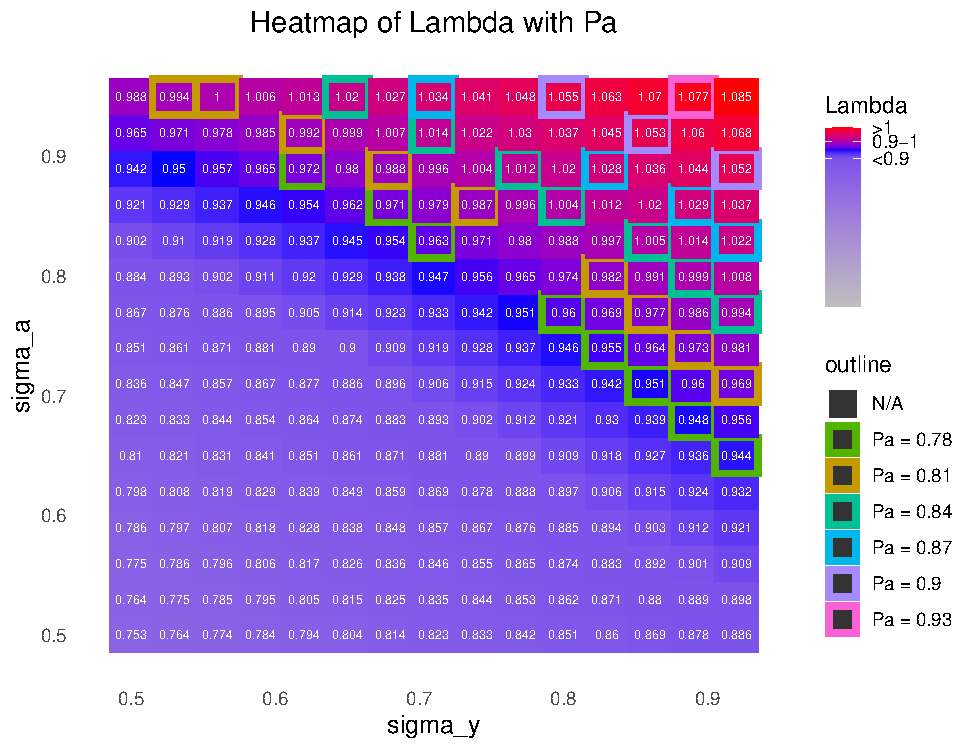
\includegraphics{sensitivity_files/figure-pdf/unnamed-chunk-7-1.pdf}

\begin{Shaded}
\begin{Highlighting}[]
\NormalTok{b\_y\_values }\OtherTok{\textless{}{-}} \FunctionTok{seq}\NormalTok{(}\FloatTok{0.5}\NormalTok{, }\FloatTok{0.9}\NormalTok{, }\AttributeTok{by =} \FloatTok{0.03}\NormalTok{)}
\NormalTok{b\_a\_values }\OtherTok{\textless{}{-}} \FunctionTok{seq}\NormalTok{(}\FloatTok{0.5}\NormalTok{, }\FloatTok{0.93}\NormalTok{, }\AttributeTok{by =} \FloatTok{0.03}\NormalTok{)}

\CommentTok{\# Initialize a data frame to store results}
\NormalTok{heatmap\_data }\OtherTok{\textless{}{-}} \FunctionTok{data.frame}\NormalTok{(}\AttributeTok{b\_a =} \FunctionTok{numeric}\NormalTok{(}\DecValTok{0}\NormalTok{), }\AttributeTok{b\_y =} \FunctionTok{numeric}\NormalTok{(}\DecValTok{0}\NormalTok{), }\AttributeTok{lam3 =} \FunctionTok{numeric}\NormalTok{(}\DecValTok{0}\NormalTok{), }\AttributeTok{b =} \FunctionTok{numeric}\NormalTok{(}\DecValTok{0}\NormalTok{))}

\CommentTok{\# Iterate through all combinations of sigma\_y and sigma\_a}
\ControlFlowTok{for}\NormalTok{ (b\_y }\ControlFlowTok{in}\NormalTok{ b\_y\_values) \{}
  \ControlFlowTok{for}\NormalTok{ (b\_a }\ControlFlowTok{in}\NormalTok{ b\_a\_values) \{}
    \CommentTok{\# Update the parameter list}
\NormalTok{    param\_list }\OtherTok{\textless{}{-}} \FunctionTok{list}\NormalTok{(}
      \AttributeTok{sigma\_y =} \FloatTok{0.8}\NormalTok{,}
      \AttributeTok{sigma\_a =} \FloatTok{0.8}\NormalTok{,}
      \AttributeTok{b\_a =}\NormalTok{ b\_a, }\CommentTok{\# example value}
      \AttributeTok{b\_y =}\NormalTok{ b\_y, }\CommentTok{\# example value}
      \AttributeTok{m =} \FloatTok{1.5}\NormalTok{,   }\CommentTok{\# example value}
      \AttributeTok{r =} \FloatTok{0.5}\NormalTok{,   }\CommentTok{\# example value}
      \AttributeTok{sigma\_j =} \FloatTok{0.45}\SpecialCharTok{\^{}}\NormalTok{(}\DecValTok{12}\SpecialCharTok{/}\DecValTok{34}\NormalTok{) }\CommentTok{\# example value}
\NormalTok{    )}
    
    \CommentTok{\# Calculate lam3 and Pa}
\NormalTok{    construct\_result }\OtherTok{\textless{}{-}} \FunctionTok{constructMatrix3}\NormalTok{(param\_list)}
\NormalTok{    b\_collapsed }\OtherTok{\textless{}{-}} \FunctionTok{param\_collapse}\NormalTok{(param\_list)}
    
    \CommentTok{\# Append the result to the data frame}
\NormalTok{    heatmap\_data }\OtherTok{\textless{}{-}} \FunctionTok{rbind}\NormalTok{(heatmap\_data, }\FunctionTok{data.frame}\NormalTok{(}
      \AttributeTok{b\_a =}\NormalTok{ b\_a,}
      \AttributeTok{b\_y =}\NormalTok{ b\_y,}
      \AttributeTok{lam3 =}\NormalTok{ construct\_result}\SpecialCharTok{$}\NormalTok{lam3,}
      \AttributeTok{b =}\NormalTok{ b\_collapsed}\SpecialCharTok{$}\NormalTok{b}
\NormalTok{    ))}
\NormalTok{  \}}
\NormalTok{\}}

\NormalTok{interest\_b }\OtherTok{\textless{}{-}} \FunctionTok{seq}\NormalTok{(}\FloatTok{0.5}\NormalTok{, }\FloatTok{0.9}\NormalTok{, }\AttributeTok{by =} \FloatTok{0.1}\NormalTok{)}

\CommentTok{\# Compare each Pa with all others and add an outline flag}
\NormalTok{heatmap\_data }\OtherTok{\textless{}{-}}\NormalTok{ heatmap\_data }\SpecialCharTok{\%\textgreater{}\%}
  \FunctionTok{mutate}\NormalTok{(}\AttributeTok{outline =} \StringTok{"N/A"}\NormalTok{) }\SpecialCharTok{\%\textgreater{}\%}  \CommentTok{\# Set default outline as "N/A"}
  \FunctionTok{mutate}\NormalTok{(}\AttributeTok{outline =} \FunctionTok{sapply}\NormalTok{(b, }\ControlFlowTok{function}\NormalTok{(current\_b) \{}
    \CommentTok{\# Check if current\_Pa is within 0.005 of any value in interest\_Pa}
\NormalTok{    matched\_b }\OtherTok{\textless{}{-}} \FunctionTok{sapply}\NormalTok{(interest\_b, }\ControlFlowTok{function}\NormalTok{(target\_b) \{}\FunctionTok{abs}\NormalTok{(current\_b }\SpecialCharTok{{-}}\NormalTok{ target\_b) }\SpecialCharTok{\textless{}=} \FloatTok{0.005}\NormalTok{\})}
    
    \CommentTok{\# If matched, return the Pa value; otherwise, return "N/A"}
    \ControlFlowTok{if}\NormalTok{ (}\FunctionTok{any}\NormalTok{(matched\_b)) \{}\FunctionTok{paste}\NormalTok{(}\StringTok{"b ="}\NormalTok{, interest\_b[}\FunctionTok{which}\NormalTok{(matched\_b)])\} }\ControlFlowTok{else}\NormalTok{ \{}\StringTok{"N/A"}\NormalTok{\}}
\NormalTok{  \}))}

\CommentTok{\# Generate a color palette for each Pa group}
\NormalTok{n\_groups }\OtherTok{\textless{}{-}} \FunctionTok{length}\NormalTok{(}\FunctionTok{unique}\NormalTok{(heatmap\_data}\SpecialCharTok{$}\NormalTok{outline))}
\NormalTok{group\_colors }\OtherTok{\textless{}{-}} \FunctionTok{setNames}\NormalTok{(scales}\SpecialCharTok{::}\FunctionTok{hue\_pal}\NormalTok{()(n\_groups), }\FunctionTok{unique}\NormalTok{(heatmap\_data}\SpecialCharTok{$}\NormalTok{outline))}

\NormalTok{group\_colors[}\StringTok{"N/A"}\NormalTok{] }\OtherTok{\textless{}{-}} \StringTok{"transparent"}

\CommentTok{\# Plot the heatmap}
\FunctionTok{ggplot}\NormalTok{(heatmap\_data, }\FunctionTok{aes}\NormalTok{(}\AttributeTok{x =}\NormalTok{ b\_y, }\AttributeTok{y =}\NormalTok{ b\_a, }\AttributeTok{fill =}\NormalTok{ lam3)) }\SpecialCharTok{+}
  \FunctionTok{geom\_tile}\NormalTok{(}\FunctionTok{aes}\NormalTok{(}\AttributeTok{color =}\NormalTok{ outline), }\AttributeTok{size =} \FloatTok{1.5}\NormalTok{) }\SpecialCharTok{+}  \CommentTok{\# Use Pa\_group for the color outline}
  \FunctionTok{geom\_text}\NormalTok{(}\FunctionTok{aes}\NormalTok{(}\AttributeTok{label =} \FunctionTok{round}\NormalTok{(lam3, }\AttributeTok{digits =} \DecValTok{3}\NormalTok{)), }\AttributeTok{color =} \StringTok{"white"}\NormalTok{, }\AttributeTok{size =} \DecValTok{2}\NormalTok{) }\SpecialCharTok{+}
  \FunctionTok{scale\_color\_manual}\NormalTok{(}\AttributeTok{values =} \FunctionTok{setNames}\NormalTok{(group\_colors, }\FunctionTok{unique}\NormalTok{(heatmap\_data}\SpecialCharTok{$}\NormalTok{outline))) }\SpecialCharTok{+}  \CommentTok{\# Apply color palette}
  \FunctionTok{scale\_fill\_gradientn}\NormalTok{(}
    \AttributeTok{colors =} \FunctionTok{c}\NormalTok{(}\StringTok{"gray"}\NormalTok{, }\StringTok{"blue"}\NormalTok{, }\StringTok{"red"}\NormalTok{), }
    \AttributeTok{values =}\NormalTok{ scales}\SpecialCharTok{::}\FunctionTok{rescale}\NormalTok{(}\FunctionTok{c}\NormalTok{(}\DecValTok{0}\NormalTok{, }\FloatTok{0.9}\NormalTok{, }\DecValTok{1}\NormalTok{, }\FloatTok{1.086}\NormalTok{)),}
    \AttributeTok{limits =} \FunctionTok{c}\NormalTok{(}\DecValTok{0}\NormalTok{, }\FloatTok{1.086}\NormalTok{),}
    \AttributeTok{breaks =} \FunctionTok{c}\NormalTok{(}\FloatTok{0.9}\NormalTok{, }\DecValTok{1}\NormalTok{, }\FloatTok{1.086}\NormalTok{),}
    \AttributeTok{labels =} \FunctionTok{c}\NormalTok{(}\StringTok{"\textless{}0.9"}\NormalTok{, }\StringTok{"0.9{-}1"}\NormalTok{, }\StringTok{"\textgreater{}1"}\NormalTok{),}
    \AttributeTok{name =} \StringTok{"Lambda"}
\NormalTok{  ) }\SpecialCharTok{+}
  \FunctionTok{labs}\NormalTok{(}\AttributeTok{x =} \StringTok{"b\_y"}\NormalTok{, }\AttributeTok{y =} \StringTok{"b\_a"}\NormalTok{, }\AttributeTok{title =} \StringTok{"Heatmap of Lambda with b"}\NormalTok{) }\SpecialCharTok{+}
  \FunctionTok{theme\_minimal}\NormalTok{() }\SpecialCharTok{+}
  \FunctionTok{theme}\NormalTok{(}
    \AttributeTok{panel.grid =} \FunctionTok{element\_blank}\NormalTok{(),}
    \AttributeTok{axis.title =} \FunctionTok{element\_text}\NormalTok{(}\AttributeTok{size =} \DecValTok{12}\NormalTok{),}
    \AttributeTok{plot.title =} \FunctionTok{element\_text}\NormalTok{(}\AttributeTok{hjust =} \FloatTok{0.5}\NormalTok{, }\AttributeTok{size =} \DecValTok{14}\NormalTok{)}
\NormalTok{  )}
\end{Highlighting}
\end{Shaded}

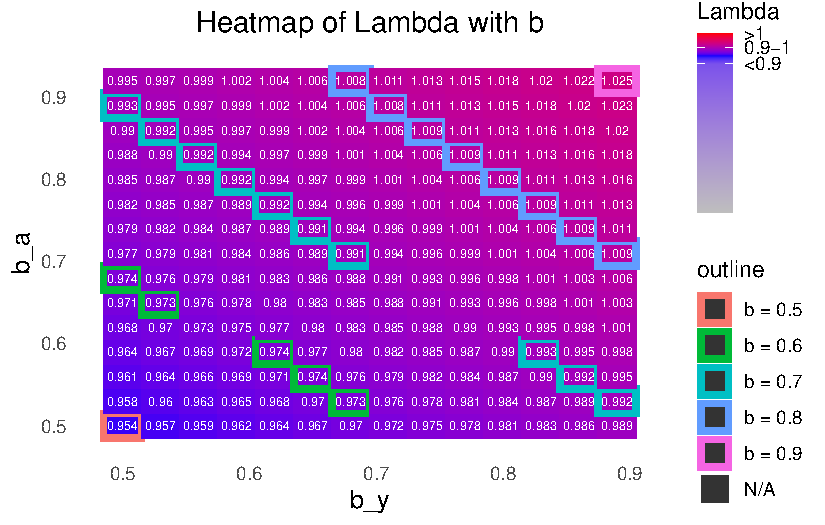
\includegraphics{sensitivity_files/figure-pdf/unnamed-chunk-8-1.pdf}

\subsection{different pairing
propensity}\label{different-pairing-propensity}

\begin{Shaded}
\begin{Highlighting}[]
\NormalTok{b\_value }\OtherTok{\textless{}{-}} \FunctionTok{seq}\NormalTok{(}\DecValTok{0}\NormalTok{, }\FloatTok{0.9}\NormalTok{, }\AttributeTok{by =} \FloatTok{0.02}\NormalTok{)}

  
\CommentTok{\# Initialize a data frame to store results}
\NormalTok{all\_b\_lam3 }\OtherTok{\textless{}{-}} \FunctionTok{data.frame}\NormalTok{(}\AttributeTok{b =} \FunctionTok{numeric}\NormalTok{(}\DecValTok{0}\NormalTok{), }\AttributeTok{lam3 =} \FunctionTok{numeric}\NormalTok{(}\DecValTok{0}\NormalTok{))}
  
\CommentTok{\# Iterate through paired combinations}
\ControlFlowTok{for}\NormalTok{ (i }\ControlFlowTok{in} \DecValTok{1}\SpecialCharTok{:}\FunctionTok{length}\NormalTok{(b\_value)) \{}
\NormalTok{  b }\OtherTok{\textless{}{-}}\NormalTok{ b\_value[i]}
\NormalTok{  hyp\_p3}\SpecialCharTok{$}\NormalTok{b\_a }\OtherTok{\textless{}{-}}\NormalTok{ b}
\NormalTok{  hyp\_p3}\SpecialCharTok{$}\NormalTok{b\_y }\OtherTok{\textless{}{-}}\NormalTok{ b}
    
  \CommentTok{\# Run constructMatrix3 and calculate lam3}
\NormalTok{  lam3 }\OtherTok{\textless{}{-}} \FunctionTok{constructMatrix3}\NormalTok{(hyp\_p3)}\SpecialCharTok{$}\NormalTok{lam3}

  \CommentTok{\# Store the current lam3 along with b}
\NormalTok{  all\_b\_lam3 }\OtherTok{\textless{}{-}} \FunctionTok{rbind}\NormalTok{(all\_b\_lam3, }\FunctionTok{data.frame}\NormalTok{(}\AttributeTok{b =}\NormalTok{ b, }\AttributeTok{lam3 =}\NormalTok{ lam3))\}}

\CommentTok{\# Calculate log sensitivity: (log difference of lam3 over log difference of b)}
\NormalTok{all\_b\_lam3}\SpecialCharTok{$}\NormalTok{log\_sensitivity }\OtherTok{\textless{}{-}} \FunctionTok{c}\NormalTok{(}\ConstantTok{NA}\NormalTok{, }\FunctionTok{diff}\NormalTok{(}\FunctionTok{log}\NormalTok{(all\_b\_lam3}\SpecialCharTok{$}\NormalTok{lam3)) }\SpecialCharTok{/} \FunctionTok{diff}\NormalTok{(}\FunctionTok{log}\NormalTok{(all\_b\_lam3}\SpecialCharTok{$}\NormalTok{b)))}

\CommentTok{\# Calculate log elasticity: (b / lam3) * log\_sensitivity}
\NormalTok{all\_b\_lam3}\SpecialCharTok{$}\NormalTok{log\_elasticity }\OtherTok{\textless{}{-}} \FunctionTok{c}\NormalTok{(}\ConstantTok{NA}\NormalTok{, (all\_b\_lam3}\SpecialCharTok{$}\NormalTok{b[}\SpecialCharTok{{-}}\DecValTok{1}\NormalTok{] }\SpecialCharTok{/}\NormalTok{ all\_b\_lam3}\SpecialCharTok{$}\NormalTok{lam3[}\SpecialCharTok{{-}}\DecValTok{1}\NormalTok{]) }\SpecialCharTok{*} \FunctionTok{diff}\NormalTok{(}\FunctionTok{log}\NormalTok{(all\_b\_lam3}\SpecialCharTok{$}\NormalTok{lam3)) }\SpecialCharTok{/} \FunctionTok{diff}\NormalTok{(}\FunctionTok{log}\NormalTok{(all\_b\_lam3}\SpecialCharTok{$}\NormalTok{b)))}

\NormalTok{b\_sensitivity\_plot }\OtherTok{\textless{}{-}} \FunctionTok{ggplot}\NormalTok{(all\_b\_lam3, }\FunctionTok{aes}\NormalTok{(}\AttributeTok{x =}\NormalTok{ b, }\AttributeTok{y =}\NormalTok{ log\_sensitivity)) }\SpecialCharTok{+}
  \FunctionTok{geom\_line}\NormalTok{(}\AttributeTok{color =} \StringTok{"red"}\NormalTok{) }\SpecialCharTok{+}
  \FunctionTok{labs}\NormalTok{(}\AttributeTok{x =} \StringTok{"breeding propensity"}\NormalTok{,}
       \AttributeTok{y =} \StringTok{"absolute sensitivity (dLam3/db)"}\NormalTok{) }\SpecialCharTok{+}
  \FunctionTok{scale\_x\_continuous}\NormalTok{(}\AttributeTok{limits =} \FunctionTok{c}\NormalTok{(}\DecValTok{0}\NormalTok{, }\FloatTok{0.9}\NormalTok{))}

\NormalTok{b\_elasticity\_plot }\OtherTok{\textless{}{-}} \FunctionTok{ggplot}\NormalTok{(all\_b\_lam3, }\FunctionTok{aes}\NormalTok{(}\AttributeTok{x =}\NormalTok{ b, }\AttributeTok{y =}\NormalTok{ log\_elasticity)) }\SpecialCharTok{+}
  \FunctionTok{geom\_line}\NormalTok{(}\AttributeTok{color =} \StringTok{"blue"}\NormalTok{) }\SpecialCharTok{+}
  \FunctionTok{labs}\NormalTok{(}\AttributeTok{x =} \StringTok{"breeding propensity"}\NormalTok{,}
       \AttributeTok{y =} \StringTok{"Elasticity"}\NormalTok{) }\SpecialCharTok{+}
  \FunctionTok{scale\_x\_continuous}\NormalTok{(}\AttributeTok{limits =} \FunctionTok{c}\NormalTok{(}\DecValTok{0}\NormalTok{, }\FloatTok{0.9}\NormalTok{))}

\NormalTok{b\_lam\_line\_plot }\OtherTok{\textless{}{-}} \FunctionTok{ggplot}\NormalTok{(all\_b\_lam3, }\FunctionTok{aes}\NormalTok{(}\AttributeTok{x =}\NormalTok{ b, }\AttributeTok{y =}\NormalTok{ lam3)) }\SpecialCharTok{+} 
  \FunctionTok{geom\_line}\NormalTok{()}\SpecialCharTok{+}
  \FunctionTok{labs}\NormalTok{(}\AttributeTok{x =} \StringTok{"breeding propensity"}\NormalTok{,}
        \AttributeTok{y =} \StringTok{"Lambda"}\NormalTok{)}\SpecialCharTok{+}
  \FunctionTok{scale\_x\_continuous}\NormalTok{(}\AttributeTok{limits =} \FunctionTok{c}\NormalTok{(}\DecValTok{0}\NormalTok{, }\FloatTok{0.9}\NormalTok{))}\SpecialCharTok{+}
  \FunctionTok{scale\_y\_continuous}\NormalTok{(}\AttributeTok{limits =} \FunctionTok{c}\NormalTok{(}\FloatTok{0.8}\NormalTok{, }\FloatTok{1.05}\NormalTok{))}

\NormalTok{params }\OtherTok{\textless{}{-}} \FunctionTok{ggplot}\NormalTok{() }\SpecialCharTok{+}
    \FunctionTok{annotate}\NormalTok{(}\StringTok{"text"}\NormalTok{, }\AttributeTok{x =} \FloatTok{0.5}\NormalTok{, }\AttributeTok{y =} \FloatTok{0.5}\NormalTok{, }
             \AttributeTok{label =} \FunctionTok{paste}\NormalTok{(}\StringTok{"m ="}\NormalTok{, hyp\_p3}\SpecialCharTok{$}\NormalTok{m, }\StringTok{"}\SpecialCharTok{\textbackslash{}n}\StringTok{"}\NormalTok{,}
                           \StringTok{"r ="}\NormalTok{,hyp\_p3}\SpecialCharTok{$}\NormalTok{r,}\StringTok{"}\SpecialCharTok{\textbackslash{}n}\StringTok{"}\NormalTok{,}
                           \StringTok{"sigma\_j ="}\NormalTok{, hyp\_p3}\SpecialCharTok{$}\NormalTok{sigma\_j,}\StringTok{"}\SpecialCharTok{\textbackslash{}n}\StringTok{"}\NormalTok{,}
                           \StringTok{"sigma\_a ="}\NormalTok{,hyp\_p3}\SpecialCharTok{$}\NormalTok{sigma\_a,}\StringTok{"}\SpecialCharTok{\textbackslash{}n}\StringTok{"}\NormalTok{,}
                           \StringTok{"sigma\_y ="}\NormalTok{,hyp\_p3}\SpecialCharTok{$}\NormalTok{sigma\_y,}\StringTok{"}\SpecialCharTok{\textbackslash{}n}\StringTok{"}\NormalTok{,}
                           \StringTok{"b 0{-}0.9"}
\NormalTok{                           ), }
             \AttributeTok{size =} \DecValTok{4}\NormalTok{, }\AttributeTok{hjust =} \FloatTok{0.5}\NormalTok{, }\AttributeTok{vjust =} \FloatTok{0.5}\NormalTok{) }\SpecialCharTok{+}
    \FunctionTok{theme\_void}\NormalTok{()}
  
\NormalTok{b\_lam\_annotated }\OtherTok{\textless{}{-}} \FunctionTok{ggarrange}\NormalTok{(b\_lam\_line\_plot,b\_sensitivity\_plot, b\_elasticity\_plot, params, }\AttributeTok{ncol =} \DecValTok{4}\NormalTok{, }\AttributeTok{nrow =} \DecValTok{1}\NormalTok{)}
\end{Highlighting}
\end{Shaded}

\subsection{different chick
production}\label{different-chick-production}

\begin{Shaded}
\begin{Highlighting}[]
\NormalTok{m\_value }\OtherTok{\textless{}{-}} \FunctionTok{seq}\NormalTok{(}\FloatTok{0.3}\NormalTok{, }\FloatTok{0.6}\NormalTok{, }\AttributeTok{by =} \FloatTok{0.02}\NormalTok{)}

  
\CommentTok{\# Initialize a data frame to store results}
\NormalTok{all\_m\_lam3 }\OtherTok{\textless{}{-}} \FunctionTok{data.frame}\NormalTok{(}\AttributeTok{m =} \FunctionTok{numeric}\NormalTok{(}\DecValTok{0}\NormalTok{), }\AttributeTok{lam3 =} \FunctionTok{numeric}\NormalTok{(}\DecValTok{0}\NormalTok{))}
  
\CommentTok{\# Iterate through paired combinations}
\ControlFlowTok{for}\NormalTok{ (i }\ControlFlowTok{in} \DecValTok{1}\SpecialCharTok{:}\FunctionTok{length}\NormalTok{(m\_value)) \{}
\NormalTok{  m }\OtherTok{\textless{}{-}}\NormalTok{ m\_value[i]}
\NormalTok{  hyp\_p3}\SpecialCharTok{$}\NormalTok{m }\OtherTok{\textless{}{-}}\NormalTok{ m}
    
  \CommentTok{\# Run constructMatrix3 and calculate lam3}
\NormalTok{  lam3 }\OtherTok{\textless{}{-}} \FunctionTok{constructMatrix3}\NormalTok{(hyp\_p3)}\SpecialCharTok{$}\NormalTok{lam3}

  \CommentTok{\# Store the current lam3 along with m}
\NormalTok{  all\_m\_lam3 }\OtherTok{\textless{}{-}} \FunctionTok{rbind}\NormalTok{(all\_m\_lam3, }\FunctionTok{data.frame}\NormalTok{(}\AttributeTok{m =}\NormalTok{ m, }\AttributeTok{lam3 =}\NormalTok{ lam3))\}}

\CommentTok{\# Calculate log sensitivity: (log difference of lam3 over log difference of m)}
\NormalTok{all\_m\_lam3}\SpecialCharTok{$}\NormalTok{log\_sensitivity }\OtherTok{\textless{}{-}} \FunctionTok{c}\NormalTok{(}\ConstantTok{NA}\NormalTok{, }\FunctionTok{diff}\NormalTok{(}\FunctionTok{log}\NormalTok{(all\_m\_lam3}\SpecialCharTok{$}\NormalTok{lam3)) }\SpecialCharTok{/} \FunctionTok{diff}\NormalTok{(}\FunctionTok{log}\NormalTok{(all\_m\_lam3}\SpecialCharTok{$}\NormalTok{m)))}

\CommentTok{\# Calculate log elasticity: (m / lam3) * log\_sensitivity}
\NormalTok{all\_m\_lam3}\SpecialCharTok{$}\NormalTok{log\_elasticity }\OtherTok{\textless{}{-}} \FunctionTok{c}\NormalTok{(}\ConstantTok{NA}\NormalTok{, (all\_m\_lam3}\SpecialCharTok{$}\NormalTok{m[}\SpecialCharTok{{-}}\DecValTok{1}\NormalTok{] }\SpecialCharTok{/}\NormalTok{ all\_m\_lam3}\SpecialCharTok{$}\NormalTok{lam3[}\SpecialCharTok{{-}}\DecValTok{1}\NormalTok{]) }\SpecialCharTok{*} \FunctionTok{diff}\NormalTok{(}\FunctionTok{log}\NormalTok{(all\_m\_lam3}\SpecialCharTok{$}\NormalTok{lam3)) }\SpecialCharTok{/} \FunctionTok{diff}\NormalTok{(}\FunctionTok{log}\NormalTok{(all\_m\_lam3}\SpecialCharTok{$}\NormalTok{m)))}

\NormalTok{m\_sensitivity\_plot }\OtherTok{\textless{}{-}} \FunctionTok{ggplot}\NormalTok{(all\_m\_lam3, }\FunctionTok{aes}\NormalTok{(}\AttributeTok{x =}\NormalTok{ m, }\AttributeTok{y =}\NormalTok{ log\_sensitivity)) }\SpecialCharTok{+}
  \FunctionTok{geom\_line}\NormalTok{(}\AttributeTok{color =} \StringTok{"red"}\NormalTok{) }\SpecialCharTok{+}
  \FunctionTok{labs}\NormalTok{(}\AttributeTok{x =} \StringTok{"chick production"}\NormalTok{,}
       \AttributeTok{y =} \StringTok{"absolute sensitivity (dLam3/dm)"}\NormalTok{) }\SpecialCharTok{+}
  \FunctionTok{scale\_x\_continuous}\NormalTok{(}\AttributeTok{limits =} \FunctionTok{c}\NormalTok{(}\DecValTok{0}\NormalTok{, }\FloatTok{0.9}\NormalTok{))}

\NormalTok{m\_elasticity\_plot }\OtherTok{\textless{}{-}} \FunctionTok{ggplot}\NormalTok{(all\_m\_lam3, }\FunctionTok{aes}\NormalTok{(}\AttributeTok{x =}\NormalTok{ m, }\AttributeTok{y =}\NormalTok{ log\_elasticity)) }\SpecialCharTok{+}
  \FunctionTok{geom\_line}\NormalTok{(}\AttributeTok{color =} \StringTok{"blue"}\NormalTok{) }\SpecialCharTok{+}
  \FunctionTok{labs}\NormalTok{(}\AttributeTok{x =} \StringTok{"chick production"}\NormalTok{,}
       \AttributeTok{y =} \StringTok{"Elasticity"}\NormalTok{) }\SpecialCharTok{+}
  \FunctionTok{scale\_x\_continuous}\NormalTok{(}\AttributeTok{limits =} \FunctionTok{c}\NormalTok{(}\DecValTok{0}\NormalTok{, }\FloatTok{0.9}\NormalTok{))}

\NormalTok{m\_lam\_line\_plot }\OtherTok{\textless{}{-}} \FunctionTok{ggplot}\NormalTok{(all\_m\_lam3, }\FunctionTok{aes}\NormalTok{(}\AttributeTok{x =}\NormalTok{ m, }\AttributeTok{y =}\NormalTok{ lam3)) }\SpecialCharTok{+} 
  \FunctionTok{geom\_line}\NormalTok{()}\SpecialCharTok{+}
  \FunctionTok{labs}\NormalTok{(}\AttributeTok{x =} \StringTok{"chick production"}\NormalTok{,}
        \AttributeTok{y =} \StringTok{"Lambda"}\NormalTok{)}\SpecialCharTok{+}
  \FunctionTok{scale\_x\_continuous}\NormalTok{(}\AttributeTok{limits =} \FunctionTok{c}\NormalTok{(}\FloatTok{0.3}\NormalTok{, }\FloatTok{0.6}\NormalTok{))}\SpecialCharTok{+}
  \FunctionTok{scale\_y\_continuous}\NormalTok{(}\AttributeTok{limits =} \FunctionTok{c}\NormalTok{(}\FloatTok{0.8}\NormalTok{, }\FloatTok{1.05}\NormalTok{))}

\NormalTok{params }\OtherTok{\textless{}{-}} \FunctionTok{ggplot}\NormalTok{() }\SpecialCharTok{+}
    \FunctionTok{annotate}\NormalTok{(}\StringTok{"text"}\NormalTok{, }\AttributeTok{x =} \FloatTok{0.5}\NormalTok{, }\AttributeTok{y =} \FloatTok{0.5}\NormalTok{, }
             \AttributeTok{label =} \FunctionTok{paste}\NormalTok{(}\StringTok{"b\_y ="}\NormalTok{, hyp\_p3}\SpecialCharTok{$}\NormalTok{b\_y, }\StringTok{"}\SpecialCharTok{\textbackslash{}n}\StringTok{"}\NormalTok{,}
                           \StringTok{"b\_a ="}\NormalTok{, hyp\_p3}\SpecialCharTok{$}\NormalTok{b\_a, }\StringTok{"}\SpecialCharTok{\textbackslash{}n}\StringTok{"}\NormalTok{,}
                           \StringTok{"r ="}\NormalTok{,hyp\_p3}\SpecialCharTok{$}\NormalTok{r,}\StringTok{"}\SpecialCharTok{\textbackslash{}n}\StringTok{"}\NormalTok{,}
                           \StringTok{"sigma\_j ="}\NormalTok{, hyp\_p3}\SpecialCharTok{$}\NormalTok{sigma\_j,}\StringTok{"}\SpecialCharTok{\textbackslash{}n}\StringTok{"}\NormalTok{,}
                           \StringTok{"sigma\_a ="}\NormalTok{,hyp\_p3}\SpecialCharTok{$}\NormalTok{sigma\_a,}\StringTok{"}\SpecialCharTok{\textbackslash{}n}\StringTok{"}\NormalTok{,}
                           \StringTok{"sigma\_y ="}\NormalTok{,hyp\_p3}\SpecialCharTok{$}\NormalTok{sigma\_y,}\StringTok{"}\SpecialCharTok{\textbackslash{}n}\StringTok{"}\NormalTok{,}
                           \StringTok{"m 0.3{-}0.6"}
\NormalTok{                           ), }
             \AttributeTok{size =} \DecValTok{4}\NormalTok{, }\AttributeTok{hjust =} \FloatTok{0.5}\NormalTok{, }\AttributeTok{vjust =} \FloatTok{0.5}\NormalTok{) }\SpecialCharTok{+}
    \FunctionTok{theme\_void}\NormalTok{()}
  
\NormalTok{m\_lam\_annotated }\OtherTok{\textless{}{-}} \FunctionTok{ggarrange}\NormalTok{(m\_lam\_line\_plot,m\_sensitivity\_plot,m\_elasticity\_plot,params, }\AttributeTok{ncol =} \DecValTok{4}\NormalTok{, }\AttributeTok{nrow =} \DecValTok{1}\NormalTok{)}
\end{Highlighting}
\end{Shaded}

\subsection{different sex-ratio}\label{different-sex-ratio}

\begin{Shaded}
\begin{Highlighting}[]
\NormalTok{r\_value }\OtherTok{\textless{}{-}} \FunctionTok{seq}\NormalTok{(}\FloatTok{0.3}\NormalTok{, }\FloatTok{0.6}\NormalTok{, }\AttributeTok{by =} \FloatTok{0.02}\NormalTok{)}

  
\CommentTok{\# Initialize a data frame to store results}
\NormalTok{all\_r\_lam3 }\OtherTok{\textless{}{-}} \FunctionTok{data.frame}\NormalTok{(}\AttributeTok{r =} \FunctionTok{numeric}\NormalTok{(}\DecValTok{0}\NormalTok{), }\AttributeTok{lam3 =} \FunctionTok{numeric}\NormalTok{(}\DecValTok{0}\NormalTok{))}
  
\CommentTok{\# Iterate through paired combinations}
\ControlFlowTok{for}\NormalTok{ (i }\ControlFlowTok{in} \DecValTok{1}\SpecialCharTok{:}\FunctionTok{length}\NormalTok{(r\_value)) \{}
\NormalTok{  r }\OtherTok{\textless{}{-}}\NormalTok{ r\_value[i]}
\NormalTok{  hyp\_p3}\SpecialCharTok{$}\NormalTok{r }\OtherTok{\textless{}{-}}\NormalTok{ r}
    
  \CommentTok{\# Run constructMatrix3 and calculate lam3}
\NormalTok{  lam3 }\OtherTok{\textless{}{-}} \FunctionTok{constructMatrix3}\NormalTok{(hyp\_p3)}\SpecialCharTok{$}\NormalTok{lam3}

  \CommentTok{\# Store the current lam3 along with r}
\NormalTok{  all\_r\_lam3 }\OtherTok{\textless{}{-}} \FunctionTok{rbind}\NormalTok{(all\_r\_lam3, }\FunctionTok{data.frame}\NormalTok{(}\AttributeTok{r =}\NormalTok{ r, }\AttributeTok{lam3 =}\NormalTok{ lam3))\}}

\CommentTok{\# Calculate log sensitivity: (log difference of lam3 over log difference of m)}
\NormalTok{all\_r\_lam3}\SpecialCharTok{$}\NormalTok{log\_sensitivity }\OtherTok{\textless{}{-}} \FunctionTok{c}\NormalTok{(}\ConstantTok{NA}\NormalTok{, }\FunctionTok{diff}\NormalTok{(}\FunctionTok{log}\NormalTok{(all\_r\_lam3}\SpecialCharTok{$}\NormalTok{lam3)) }\SpecialCharTok{/} \FunctionTok{diff}\NormalTok{(}\FunctionTok{log}\NormalTok{(all\_r\_lam3}\SpecialCharTok{$}\NormalTok{r)))}

\CommentTok{\# Calculate log elasticity: (m / lam3) * log\_sensitivity}
\NormalTok{all\_r\_lam3}\SpecialCharTok{$}\NormalTok{log\_elasticity }\OtherTok{\textless{}{-}} \FunctionTok{c}\NormalTok{(}\ConstantTok{NA}\NormalTok{, (all\_r\_lam3}\SpecialCharTok{$}\NormalTok{r[}\SpecialCharTok{{-}}\DecValTok{1}\NormalTok{] }\SpecialCharTok{/}\NormalTok{ all\_r\_lam3}\SpecialCharTok{$}\NormalTok{lam3[}\SpecialCharTok{{-}}\DecValTok{1}\NormalTok{]) }\SpecialCharTok{*} \FunctionTok{diff}\NormalTok{(}\FunctionTok{log}\NormalTok{(all\_r\_lam3}\SpecialCharTok{$}\NormalTok{lam3)) }\SpecialCharTok{/} \FunctionTok{diff}\NormalTok{(}\FunctionTok{log}\NormalTok{(all\_r\_lam3}\SpecialCharTok{$}\NormalTok{r)))}

\NormalTok{r\_sensitivity\_plot }\OtherTok{\textless{}{-}} \FunctionTok{ggplot}\NormalTok{(all\_r\_lam3, }\FunctionTok{aes}\NormalTok{(}\AttributeTok{x =}\NormalTok{ r, }\AttributeTok{y =}\NormalTok{ log\_sensitivity)) }\SpecialCharTok{+}
  \FunctionTok{geom\_line}\NormalTok{(}\AttributeTok{color =} \StringTok{"red"}\NormalTok{) }\SpecialCharTok{+}
  \FunctionTok{labs}\NormalTok{(}\AttributeTok{x =} \StringTok{"sex ratio"}\NormalTok{,}
       \AttributeTok{y =} \StringTok{"absolute sensitivity (dLam3/dm)"}\NormalTok{) }\SpecialCharTok{+}
  \FunctionTok{scale\_x\_continuous}\NormalTok{(}\AttributeTok{limits =} \FunctionTok{c}\NormalTok{(}\DecValTok{0}\NormalTok{, }\FloatTok{0.9}\NormalTok{))}

\NormalTok{r\_elasticity\_plot }\OtherTok{\textless{}{-}} \FunctionTok{ggplot}\NormalTok{(all\_r\_lam3, }\FunctionTok{aes}\NormalTok{(}\AttributeTok{x =}\NormalTok{ r, }\AttributeTok{y =}\NormalTok{ log\_elasticity)) }\SpecialCharTok{+}
  \FunctionTok{geom\_line}\NormalTok{(}\AttributeTok{color =} \StringTok{"blue"}\NormalTok{) }\SpecialCharTok{+}
  \FunctionTok{labs}\NormalTok{(}\AttributeTok{x =} \StringTok{"sex ratio"}\NormalTok{,}
       \AttributeTok{y =} \StringTok{"Elasticity"}\NormalTok{) }\SpecialCharTok{+}
  \FunctionTok{scale\_x\_continuous}\NormalTok{(}\AttributeTok{limits =} \FunctionTok{c}\NormalTok{(}\DecValTok{0}\NormalTok{, }\FloatTok{0.9}\NormalTok{))}

\NormalTok{r\_lam\_line\_plot }\OtherTok{\textless{}{-}} \FunctionTok{ggplot}\NormalTok{(all\_r\_lam3, }\FunctionTok{aes}\NormalTok{(}\AttributeTok{x =}\NormalTok{ r, }\AttributeTok{y =}\NormalTok{ lam3)) }\SpecialCharTok{+} 
  \FunctionTok{geom\_line}\NormalTok{()}\SpecialCharTok{+}
  \FunctionTok{labs}\NormalTok{(}\AttributeTok{x =} \StringTok{"sex ratio"}\NormalTok{,}
        \AttributeTok{y =} \StringTok{"Lambda"}\NormalTok{)}\SpecialCharTok{+}
  \FunctionTok{scale\_x\_continuous}\NormalTok{(}\AttributeTok{limits =} \FunctionTok{c}\NormalTok{(}\FloatTok{0.3}\NormalTok{, }\FloatTok{0.6}\NormalTok{))}\SpecialCharTok{+}
  \FunctionTok{scale\_y\_continuous}\NormalTok{(}\AttributeTok{limits =} \FunctionTok{c}\NormalTok{(}\FloatTok{0.8}\NormalTok{, }\FloatTok{1.05}\NormalTok{))}
\NormalTok{params }\OtherTok{\textless{}{-}} \FunctionTok{ggplot}\NormalTok{() }\SpecialCharTok{+}
    \FunctionTok{annotate}\NormalTok{(}\StringTok{"text"}\NormalTok{, }\AttributeTok{x =} \FloatTok{0.5}\NormalTok{, }\AttributeTok{y =} \FloatTok{0.5}\NormalTok{, }
             \AttributeTok{label =} \FunctionTok{paste}\NormalTok{(}\StringTok{"b\_y ="}\NormalTok{, hyp\_p3}\SpecialCharTok{$}\NormalTok{b\_y, }\StringTok{"}\SpecialCharTok{\textbackslash{}n}\StringTok{"}\NormalTok{,}
                           \StringTok{"b\_a ="}\NormalTok{, hyp\_p3}\SpecialCharTok{$}\NormalTok{b\_a, }\StringTok{"}\SpecialCharTok{\textbackslash{}n}\StringTok{"}\NormalTok{,}
                           \StringTok{"m ="}\NormalTok{,hyp\_p3}\SpecialCharTok{$}\NormalTok{m,}\StringTok{"}\SpecialCharTok{\textbackslash{}n}\StringTok{"}\NormalTok{,}
                           \StringTok{"sigma\_j ="}\NormalTok{, hyp\_p3}\SpecialCharTok{$}\NormalTok{sigma\_j,}\StringTok{"}\SpecialCharTok{\textbackslash{}n}\StringTok{"}\NormalTok{,}
                           \StringTok{"sigma\_a ="}\NormalTok{,hyp\_p3}\SpecialCharTok{$}\NormalTok{sigma\_a,}\StringTok{"}\SpecialCharTok{\textbackslash{}n}\StringTok{"}\NormalTok{,}
                           \StringTok{"sigma\_y ="}\NormalTok{,hyp\_p3}\SpecialCharTok{$}\NormalTok{sigma\_y,}\StringTok{"}\SpecialCharTok{\textbackslash{}n}\StringTok{"}\NormalTok{,}
                           \StringTok{"r 0.3{-}0.6"}
\NormalTok{                           ), }
             \AttributeTok{size =} \DecValTok{4}\NormalTok{, }\AttributeTok{hjust =} \FloatTok{0.5}\NormalTok{, }\AttributeTok{vjust =} \FloatTok{0.5}\NormalTok{) }\SpecialCharTok{+}
    \FunctionTok{theme\_void}\NormalTok{()}
  
\NormalTok{r\_lam\_annotated }\OtherTok{\textless{}{-}} \FunctionTok{ggarrange}\NormalTok{(r\_lam\_line\_plot,r\_sensitivity\_plot, r\_elasticity\_plot, params, }\AttributeTok{ncol =} \DecValTok{4}\NormalTok{, }\AttributeTok{nrow =} \DecValTok{1}\NormalTok{)}
\end{Highlighting}
\end{Shaded}

\subsection{different juvenile
survival}\label{different-juvenile-survival}

\begin{Shaded}
\begin{Highlighting}[]
\NormalTok{s }\OtherTok{\textless{}{-}} \FunctionTok{seq}\NormalTok{(}\FloatTok{0.2}\NormalTok{, }\FloatTok{0.5}\NormalTok{, }\AttributeTok{by =} \FloatTok{0.02}\NormalTok{)}
\NormalTok{sigma\_j\_value }\OtherTok{\textless{}{-}}\NormalTok{ s}\SpecialCharTok{\^{}}\NormalTok{(}\DecValTok{12}\SpecialCharTok{/}\DecValTok{34}\NormalTok{)}

  
\CommentTok{\# Initialize a data frame to store results}
\NormalTok{all\_sigma\_j\_lam3 }\OtherTok{\textless{}{-}} \FunctionTok{data.frame}\NormalTok{(}\AttributeTok{sigma\_j =} \FunctionTok{numeric}\NormalTok{(}\DecValTok{0}\NormalTok{), }\AttributeTok{lam3 =} \FunctionTok{numeric}\NormalTok{(}\DecValTok{0}\NormalTok{))}
  
\CommentTok{\# Iterate through paired combinations}
\ControlFlowTok{for}\NormalTok{ (i }\ControlFlowTok{in} \DecValTok{1}\SpecialCharTok{:}\FunctionTok{length}\NormalTok{(sigma\_j\_value)) \{}
\NormalTok{  sigma\_j }\OtherTok{\textless{}{-}}\NormalTok{ sigma\_j\_value[i]}
\NormalTok{  hyp\_p3}\SpecialCharTok{$}\NormalTok{sigma\_j }\OtherTok{\textless{}{-}}\NormalTok{ sigma\_j}
    
  \CommentTok{\# Run constructMatrix3 and calculate lam3}
\NormalTok{  lam3 }\OtherTok{\textless{}{-}} \FunctionTok{constructMatrix3}\NormalTok{(hyp\_p3)}\SpecialCharTok{$}\NormalTok{lam3}

  \CommentTok{\# Store the current lam3 along with r}
\NormalTok{  all\_sigma\_j\_lam3 }\OtherTok{\textless{}{-}} \FunctionTok{rbind}\NormalTok{(all\_sigma\_j\_lam3, }\FunctionTok{data.frame}\NormalTok{(}\AttributeTok{sigma\_j =}\NormalTok{ sigma\_j, }\AttributeTok{lam3 =}\NormalTok{ lam3))\}}

\CommentTok{\# Calculate log sensitivity: (log difference of lam3 over log difference of m)}
\NormalTok{all\_sigma\_j\_lam3}\SpecialCharTok{$}\NormalTok{log\_sensitivity }\OtherTok{\textless{}{-}} \FunctionTok{c}\NormalTok{(}\ConstantTok{NA}\NormalTok{, }\FunctionTok{diff}\NormalTok{(}\FunctionTok{log}\NormalTok{(all\_sigma\_j\_lam3}\SpecialCharTok{$}\NormalTok{lam3)) }\SpecialCharTok{/} \FunctionTok{diff}\NormalTok{(}\FunctionTok{log}\NormalTok{(all\_sigma\_j\_lam3}\SpecialCharTok{$}\NormalTok{sigma\_j)))}

\CommentTok{\# Calculate log elasticity: (m / lam3) * log\_sensitivity}
\NormalTok{all\_sigma\_j\_lam3}\SpecialCharTok{$}\NormalTok{log\_elasticity }\OtherTok{\textless{}{-}} \FunctionTok{c}\NormalTok{(}\ConstantTok{NA}\NormalTok{, (all\_sigma\_j\_lam3}\SpecialCharTok{$}\NormalTok{sigma\_j[}\SpecialCharTok{{-}}\DecValTok{1}\NormalTok{] }\SpecialCharTok{/}\NormalTok{ all\_sigma\_j\_lam3}\SpecialCharTok{$}\NormalTok{lam3[}\SpecialCharTok{{-}}\DecValTok{1}\NormalTok{]) }\SpecialCharTok{*} \FunctionTok{diff}\NormalTok{(}\FunctionTok{log}\NormalTok{(all\_sigma\_j\_lam3}\SpecialCharTok{$}\NormalTok{lam3)) }\SpecialCharTok{/} \FunctionTok{diff}\NormalTok{(}\FunctionTok{log}\NormalTok{(all\_sigma\_j\_lam3}\SpecialCharTok{$}\NormalTok{sigma\_j)))}

\NormalTok{sigma\_j\_sensitivity\_plot }\OtherTok{\textless{}{-}} \FunctionTok{ggplot}\NormalTok{(all\_sigma\_j\_lam3, }\FunctionTok{aes}\NormalTok{(}\AttributeTok{x =}\NormalTok{ sigma\_j, }\AttributeTok{y =}\NormalTok{ log\_sensitivity)) }\SpecialCharTok{+}
  \FunctionTok{geom\_line}\NormalTok{(}\AttributeTok{color =} \StringTok{"red"}\NormalTok{) }\SpecialCharTok{+}
  \FunctionTok{labs}\NormalTok{(}\AttributeTok{x =} \StringTok{"juvenile survival"}\NormalTok{,}
       \AttributeTok{y =} \StringTok{"absolute sensitivity (dLam3/dm)"}\NormalTok{) }\SpecialCharTok{+}
  \FunctionTok{scale\_x\_continuous}\NormalTok{(}\AttributeTok{limits =} \FunctionTok{c}\NormalTok{(}\DecValTok{0}\NormalTok{, }\FloatTok{0.9}\NormalTok{))}

\NormalTok{sigma\_j\_elasticity\_plot }\OtherTok{\textless{}{-}} \FunctionTok{ggplot}\NormalTok{(all\_sigma\_j\_lam3, }\FunctionTok{aes}\NormalTok{(}\AttributeTok{x =}\NormalTok{ sigma\_j, }\AttributeTok{y =}\NormalTok{ log\_elasticity)) }\SpecialCharTok{+}
  \FunctionTok{geom\_line}\NormalTok{(}\AttributeTok{color =} \StringTok{"blue"}\NormalTok{) }\SpecialCharTok{+}
  \FunctionTok{labs}\NormalTok{(}\AttributeTok{x =} \StringTok{"juvenile survival"}\NormalTok{,}
       \AttributeTok{y =} \StringTok{"Elasticity"}\NormalTok{) }\SpecialCharTok{+}
  \FunctionTok{scale\_x\_continuous}\NormalTok{(}\AttributeTok{limits =} \FunctionTok{c}\NormalTok{(}\DecValTok{0}\NormalTok{, }\FloatTok{0.9}\NormalTok{))}

\NormalTok{sigma\_j\_lam\_line\_plot }\OtherTok{\textless{}{-}} \FunctionTok{ggplot}\NormalTok{(all\_sigma\_j\_lam3, }\FunctionTok{aes}\NormalTok{(}\AttributeTok{x =}\NormalTok{ sigma\_j, }\AttributeTok{y =}\NormalTok{ lam3)) }\SpecialCharTok{+} 
  \FunctionTok{geom\_line}\NormalTok{()}\SpecialCharTok{+}
  \FunctionTok{labs}\NormalTok{(}\AttributeTok{x =} \StringTok{"juvenile survival"}\NormalTok{,}
        \AttributeTok{y =} \StringTok{"Lambda"}\NormalTok{)}\SpecialCharTok{+}
  \FunctionTok{scale\_x\_continuous}\NormalTok{(}\AttributeTok{limits =} \FunctionTok{c}\NormalTok{(}\FunctionTok{min}\NormalTok{(sigma\_j\_value), }\FunctionTok{max}\NormalTok{(sigma\_j\_value)))}\SpecialCharTok{+}
  \FunctionTok{scale\_y\_continuous}\NormalTok{(}\AttributeTok{limits =} \FunctionTok{c}\NormalTok{(}\FloatTok{0.8}\NormalTok{, }\FloatTok{1.05}\NormalTok{))}

\NormalTok{params }\OtherTok{\textless{}{-}} \FunctionTok{ggplot}\NormalTok{() }\SpecialCharTok{+}
    \FunctionTok{annotate}\NormalTok{(}\StringTok{"text"}\NormalTok{, }\AttributeTok{x =} \FloatTok{0.5}\NormalTok{, }\AttributeTok{y =} \FloatTok{0.5}\NormalTok{, }
             \AttributeTok{label =} \FunctionTok{paste}\NormalTok{(}\StringTok{"b\_y ="}\NormalTok{, hyp\_p3}\SpecialCharTok{$}\NormalTok{b\_y, }\StringTok{"}\SpecialCharTok{\textbackslash{}n}\StringTok{"}\NormalTok{,}
                           \StringTok{"b\_a ="}\NormalTok{, hyp\_p3}\SpecialCharTok{$}\NormalTok{b\_a, }\StringTok{"}\SpecialCharTok{\textbackslash{}n}\StringTok{"}\NormalTok{,}
                           \StringTok{"m ="}\NormalTok{,hyp\_p3}\SpecialCharTok{$}\NormalTok{m,}\StringTok{"}\SpecialCharTok{\textbackslash{}n}\StringTok{"}\NormalTok{,}
                           \StringTok{"r ="}\NormalTok{, hyp\_p3}\SpecialCharTok{$}\NormalTok{r,}\StringTok{"}\SpecialCharTok{\textbackslash{}n}\StringTok{"}\NormalTok{,}
                           \StringTok{"sigma\_a ="}\NormalTok{,hyp\_p3}\SpecialCharTok{$}\NormalTok{sigma\_a,}\StringTok{"}\SpecialCharTok{\textbackslash{}n}\StringTok{"}\NormalTok{,}
                           \StringTok{"sigma\_y ="}\NormalTok{,hyp\_p3}\SpecialCharTok{$}\NormalTok{sigma\_y,}\StringTok{"}\SpecialCharTok{\textbackslash{}n}\StringTok{"}\NormalTok{,}
                           \StringTok{"sigma\_j 0.57{-}0.78"}
\NormalTok{                           ), }
             \AttributeTok{size =} \DecValTok{4}\NormalTok{, }\AttributeTok{hjust =} \FloatTok{0.5}\NormalTok{, }\AttributeTok{vjust =} \FloatTok{0.5}\NormalTok{) }\SpecialCharTok{+}
    \FunctionTok{theme\_void}\NormalTok{()}
  
\NormalTok{sigma\_j\_lam\_annotated }\OtherTok{\textless{}{-}} \FunctionTok{ggarrange}\NormalTok{(sigma\_j\_lam\_line\_plot,sigma\_j\_sensitivity\_plot,sigma\_j\_elasticity\_plot, params, }\AttributeTok{ncol =} \DecValTok{4}\NormalTok{, }\AttributeTok{nrow =} \DecValTok{1}\NormalTok{)}
\end{Highlighting}
\end{Shaded}

\begin{Shaded}
\begin{Highlighting}[]
\FunctionTok{ggarrange}\NormalTok{(b\_lam\_annotated,}
\NormalTok{          m\_lam\_annotated,}
\NormalTok{          r\_lam\_annotated,}
\NormalTok{          sigma\_j\_lam\_annotated,}
          \AttributeTok{ncol =} \DecValTok{1}\NormalTok{, }\AttributeTok{nrow =} \DecValTok{4}\NormalTok{)}
\end{Highlighting}
\end{Shaded}

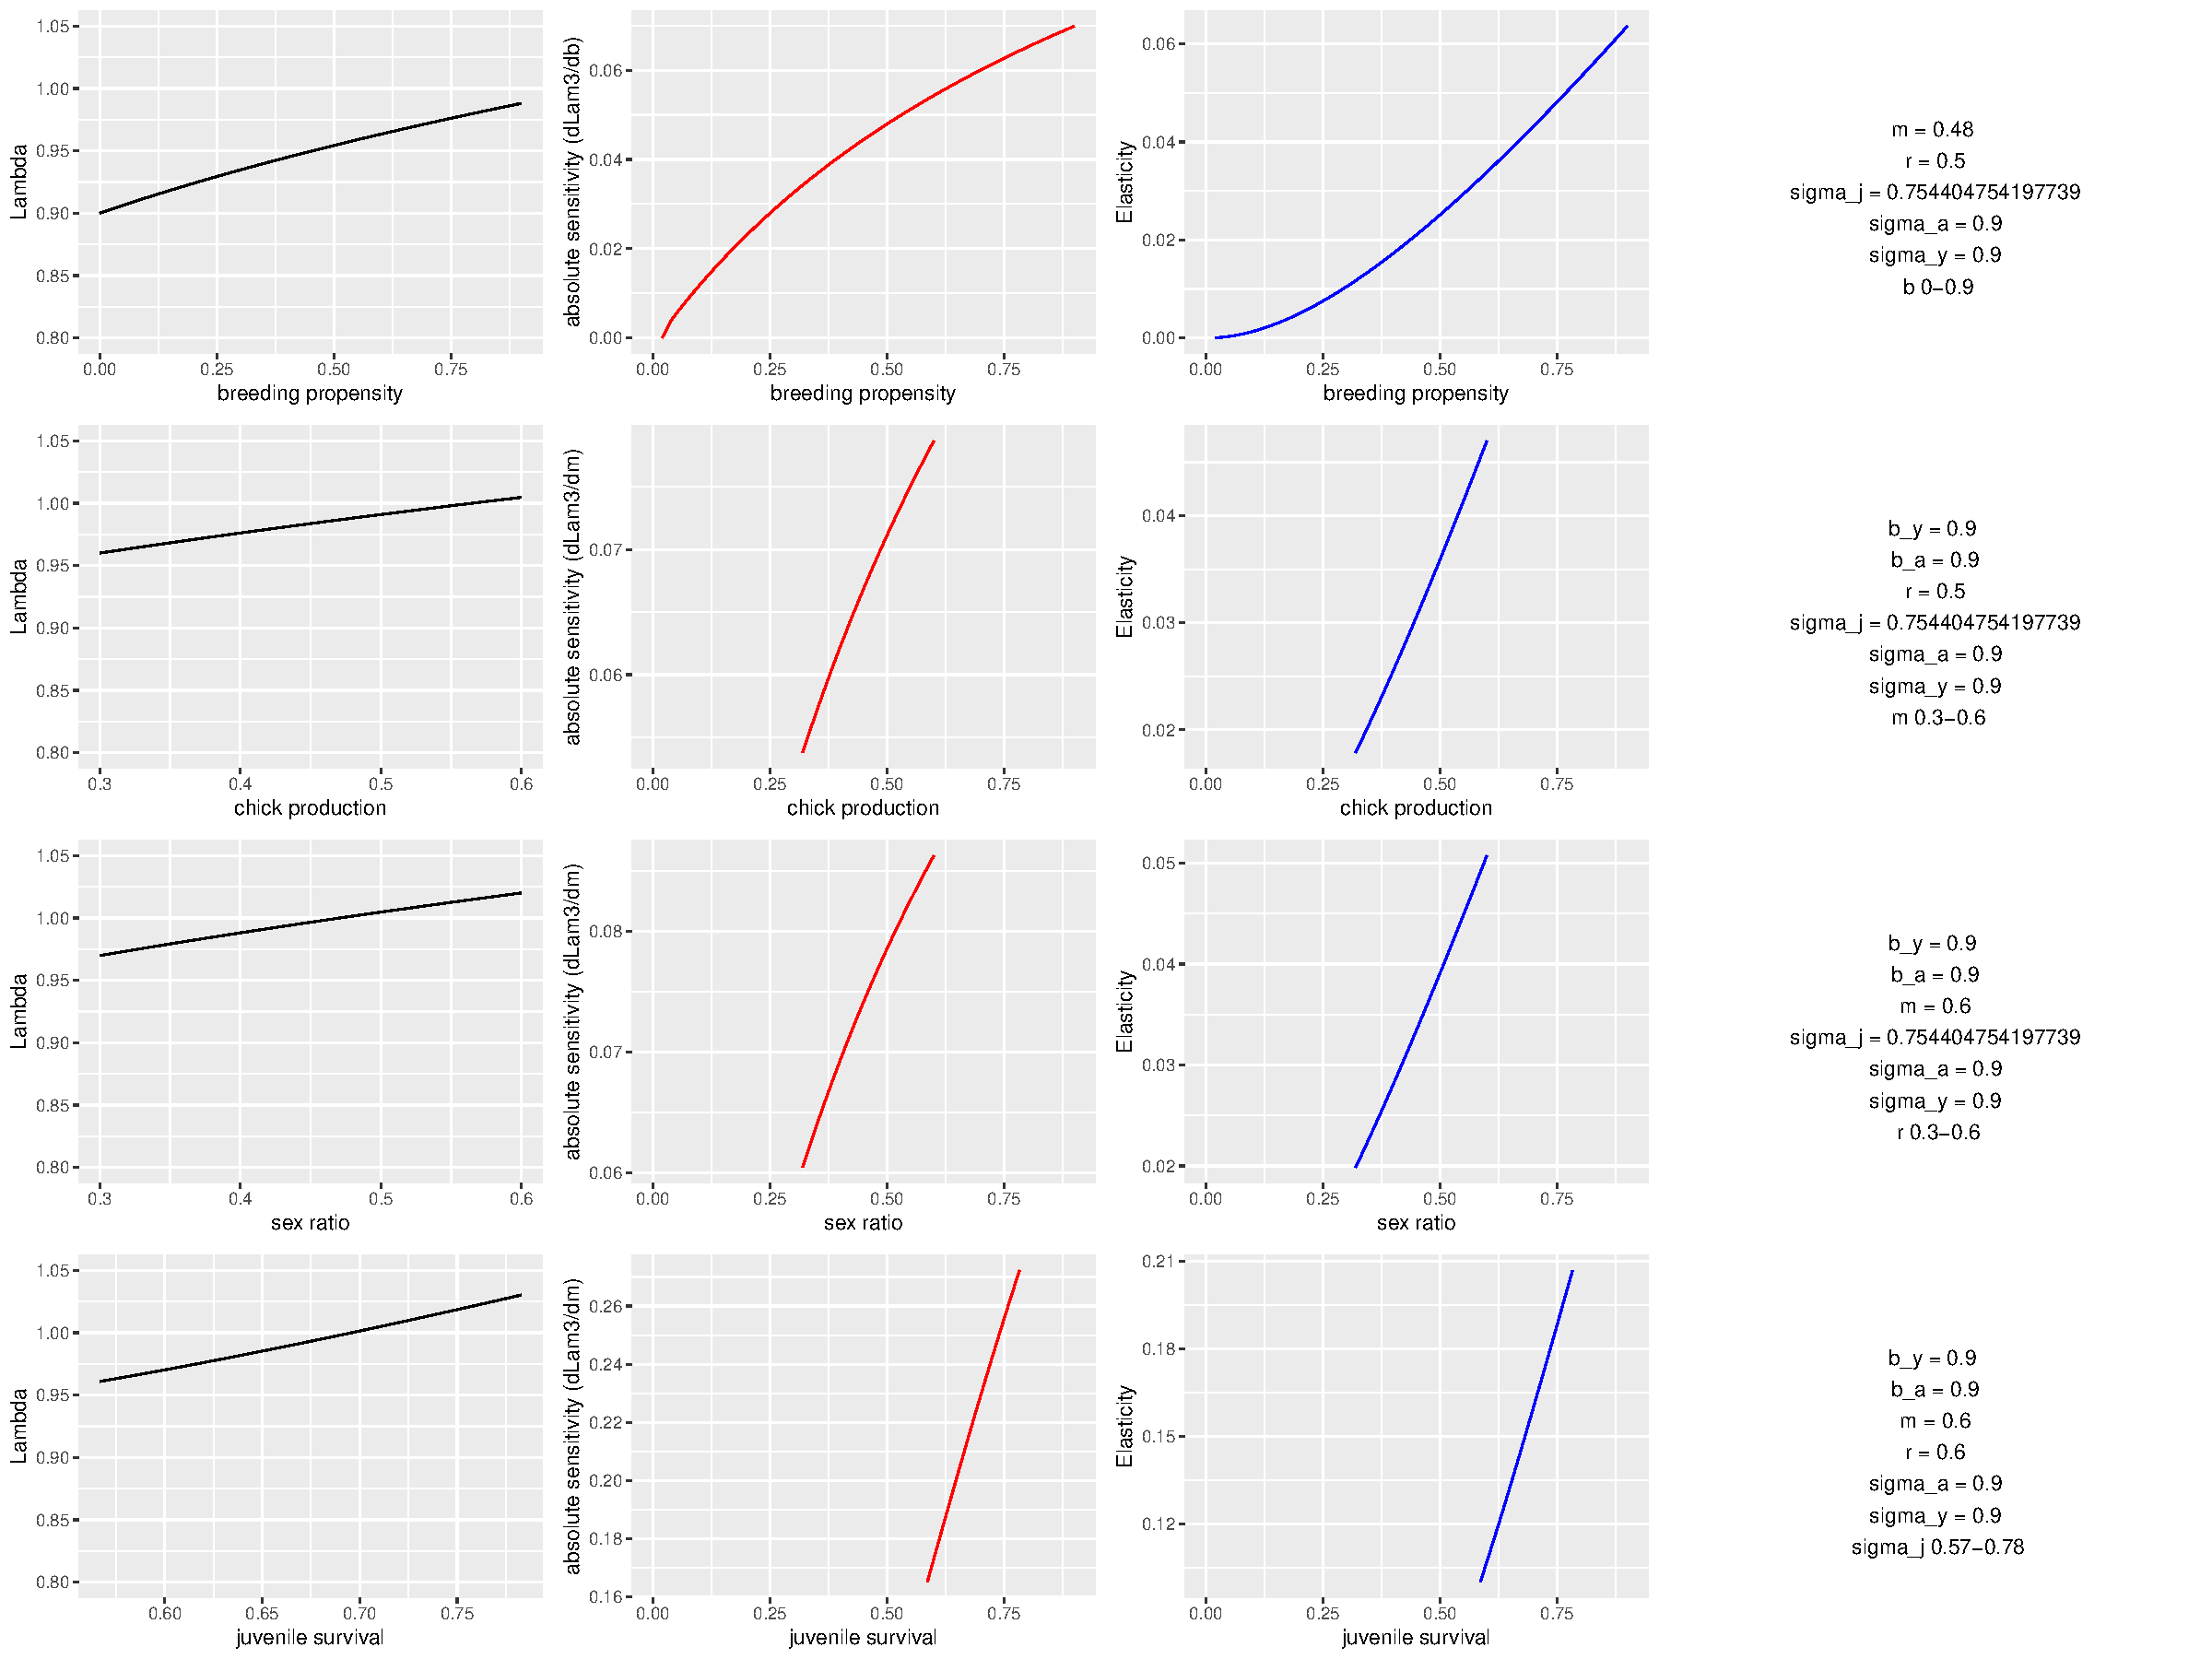
\includegraphics{sensitivity_files/figure-pdf/unnamed-chunk-13-1.pdf}




\end{document}
